\chapter{Una teoría de la memoria para secuencias binarias: evidencia de un algoritmo de compresión mental en humanos}

\section{Introducción}

%Sequence processing, the ability to encode and represent in memory a temporally ordered series of discrete elements, plays a central role in numerous human activities, including language. In the 1950’s, Karl Lashley (1) and Noam Chomsky (2) famously argued that the sequential structures that humans produce and remember cannot be reduced to mere associations of consecutive items, as envisaged in the associative theories characteristic of the Skinnerian paradigm, but must be mentally represented as recursively nested structures. The syntax of language, for instance, involves a recursive grammar of potentially unlimited embeddings of phrases within phrases, and a similar argument has been made for a “musical grammar” (3). Here, we formulate and test the theory that a similar code is needed to account for the much simpler case of binary sequences, i.e. sequences composed of two items A and B (e.g. high and low pitch tones, or red and green dots). We present experimental evidence that, even in this simple case, which can be considered as the simplest possible form of “music”, a similar postulation of nested structures is required in order to account for human memory performance. 

El procesamiento de secuencias, la capacidad de codificar y representar en la memoria una serie de elementos discretos ordenados temporalmente, juega un papel central en numerosas actividades humanas, incluido el lenguaje. En la década de 1950, Karl Lashley \cite{f1} y Noam Chomsky \cite{f2} argumentaron que las estructuras secuenciales que los humanos producen y recuerdan no pueden reducirse a meras asociaciones de elementos consecutivos, como se prevé en las teorías asociativas típicas del paradigma Skinneriano, sino que deben ser representadas mentalmente como estructuras recursivamente anidadas. La sintaxis del lenguaje, por ejemplo, implica una gramática recursiva con potencialmente infinitas inserciones de frases dentro de frases, y un argumento similar se ha propuesto para la \textit{gramática musical} \cite{f3}. En este capítulo, formulamos y probamos la teoría de que es necesario un código similar para dar cuenta de un caso más simple de representación: las secuencias binarias. Es decir, secuencias compuestas por dos elementos A y B (por ejemplo, tonos altos y bajos, o puntos rojos y verdes). Presentamos evidencia experimental de que, incluso en este caso simple (que podría considerarse como una de las formas más simples de ``música'', se requiere un postulado similar de estructuras anidadas para explicar el desempeño de la memoria humana.

%Understanding how humans and other animals encode and represent temporal sequences has recently emerged as a crucial issue in the study of comparative cognition, as it allows a direct comparison between species and therefore a test of theories of human uniqueness (4,5). Recursive phrase structures have been proposed to lie at the core of the human language faculty (6), and a competence for nested trees has been postulated to underlie several other human cognitive abilities such as mathematics or music (4,7–9). According to a recent review (4), non-human animals may encode sequences using a variety of encoding schemes, including transition probabilities, ordinal regularities (what comes first, second, etc.), recurring chunks, and algebraic patterns (10–14). However, several authors hypothesize that only humans have access to a language-like representation of nested trees (4,8), also being described as a “universal generative faculty” (9) or “language of thought” (15) capable of encoding arbitrarily nested rules.

La comprensión de cómo los humanos y otros animales codifican y representan secuencias temporales ha surgido recientemente como un tema crucial en el estudio de la cognición, ya que permite una comparación directa entre especies y, por lo tanto, una prueba de las teorías de la singularidad humana \cite{f4,f5}. Se ha propuesto que estructuras de frases recursivas se encuentran en el centro de la capacidad del lenguaje humano \cite{f6}, y se ha postulado incluso que la capacidad de manejar estructuras anidadas de representación es la base de varias habilidades cognitivas humanas como las matemáticas o la música \cite{f4,f7,f8,f9}. De acuerdo con una reciente revisión \cite{f4}, los animales no humanos podrían codificar secuencias usando una variedad de esquemas de codificación, incluyendo transiciones de probabilidad, regularidades ordinales (lo que viene primero, segundo, etc.), fragmentos recurrentes, y patrones algebraicos \cite{f10,f11,f12,f13,f14}. Sin embargo, varios autores plantean la hipótesis de que sólo los humanos tienen acceso a una representación en lenguajes de árboles anidados \cite{f4,f8}, siendo también descrita como una \textit{facultad generativa universal} \cite{f9} o \textit{lenguaje del pensamiento (del inglés LoT)} \cite{fodor1975language} capa de codificar reglas anidadas arbitrariamente. 

%Here we propose a principled language capable of encoding any arbitrary nesting of repetition and alternation structures, and we test the hypothesis that humans spontaneously encode sequences using the nested tree structures of this language. We do so using the simplest form of temporal sequences, namely binary sequences. Indeed, while the use of recursive chunking and embedding strategies is well accepted for richer sequences (e.g., language, music, or even memorizing a phone number (16)), it is not clear whether these mechanisms only become necessary at a certain level of complexity, or whether they lie at the core of human sequence processing and are therefore spontaneously employed even with the most basic forms of sequences. In addition to being the simplest possible such form, binary sequences also present several advantages. As opposed to more complex sequences, such as the ones of the natural language, which involve numerous factors that are difficult to control (prior knowledge, semantic content, word frequency, etc.), they allow to easily control the information content of the input. Furthermore, they are potentially accessible to a wide variety of populations beyond human adults, including infants and non-human primates. As such, they may provide an essential benchmark in research on the existence of a human-specific sequence processing ability. Finally, binary sequences are also widely used to study the cognitive processes and brain mechanisms involved in the perception of randomness and in statistical learning (17–22). While minimal, they nevertheless preserve the possibility of forming structures at different hierarchical levels, from simple chunking to language-like rules, and thus of arbitrating between different models of sequence encoding.

En este capítulo propones un lenguaje capaz de codificar cualquier anidamiento arbitrario de estructuras de repetición y de alternancia, y probamos la hipótesis que los seres humanos espontáneamente codifican secuencias usando las estructuras de árboles anidados de este lenguaje. Lo hacemos utilizando la forma más simple de secuencias temporales, a saber, las secuencias binarias. En efecto, mientras que el uso de técnicas recursivas de fragmentación en partes y de incrustación de estructuras está bien aceptado para secuencias más complejas (por ejemplo, el lenguaje, la música o incluso memorizar un número de teléfono \cite{f16}), no está claro si estos mecanismos sólo se vuelven necesarios a partir de un determinado nivel de complejidad, o si encuentran en el centro del procesamiento de secuencias en los humanos y, por lo tanto, se emplean de manera espontánea incluso con las formas más básicas de secuencias. Las secuencias binarias, además de ser la forma más simple de secuencias, también presentan otras varias ventajas. A diferencia de secuencias más complejas (como el lenguaje natural) que implican factores más difíciles de controlar (conocimiento previo, contenido semántico, frecuencia de palabras, etc.), las secuencias binarias permiten controlar fácilmente el contenido de información de la entrada. Además, son potencialmente accesibles a una amplia variedad de poblaciones más allá de los adultos humanos, incluyendo infantes y primates no humanos. Como tales, pueden proporcionar un punto de referencia esencial en la investigación sobre la existencia de una capacidad de procesamiento de secuencias específicas para los humanos. Finalmente, las secuencias binarias también se utilizan ampliamente para estudiar los procesos cognitivos y los mecanismos cerebrales implicados en la percepción de la aleatoriedad y en el aprendizaje estadístico \cite{f17,f18,f19,f20,f21,f22}. Aunque mínimas, conservan la posibilidad de formar estructuras en diferentes niveles jerárquicos, desde la identificación de fragmentos a reglas gramaticales, y por lo tanto de arbitrar entre diferentes modelos de codificación de las secuencias. 

\subsection{Una breve revisión de teorías y experimentos sobre la complejidad de secuencias}

%The concept of compression in working memory has a long history. Much research shows that human memory is not simply determined by the number of words, digits or locations that must be remembered, but also by their capacity to be “compressed” into a smaller number of known phrases, groups, or chunks (23–29). The apparent discrepancies between the different limits of working memory capacity proposed in the past, e.g. 7±2 items (29) versus 4 items (25,30) can indeed be reconciled if one takes into account the possibility of constituting chunks rather than encoding a complete series of individual items (16,31). The formation of chunks can be seen as a data compression process, and it was proposed that the complexity of a sequence can be defined as the size of its most compressed representation (16,32–34). 

El concepto de compresión en la memoria de trabajo tiene una larga historia. Muchas investigaciones muestran que la memoria humana no está simplemente determinada por el número de palabras, dígitos o ubicaciones que deben recordarse, sino también por su capacidad para ser \textit{comprimidos} en un número menor de frases, grupos o fragmentos conocidos \cite{f23,f24,f25,f26,f27,f28,f29}. Las aparentes discrepancias entre los diferentes límites de la capacidad de memoria de trabajo propuestos en el pasado, por ejemplo, 7 $\pm$ 2 elementos \cite{f29} frente a 4 elementos \cite{f25,f30} pueden de hecho ser reconciliados si se tiene en cuenta la posibilidad de construir fragmentos en vez de codificar una serie completa de elementos individuales \cite{f16,f31}. La formación de fragmentos puede verse como un proceso de compresión de datos, y se ha propuesto que la complejidad de una secuencia se puede definir como el tamaño de su representación más comprimida \cite{f16,f32,f33,f34}.

%Experimentally, half a century of behavioral studies has shown that accuracy in sequence encoding and production tasks varies according to the compressibility of the sequence. Glanzer and Clark (35) already proposed to use the length of the most compact description of a sequence as a measure of its complexity. They found that the number of words that participants used to describe an array of eight binary items (colored symbols) was correlated with the accuracy in reproducing it. Such mean verbalization length (MVL) predicted behavior better than a simple count of the number of runs in the sequence (e.g. “AAABBBAA” has three runs), particularly for the “ABABABAB”, which could be simply described as “alternating”. 

Experimentalmente, medio siglo de estudios de comportamiento han demostrado que la precisión en tareas de codificación y producción de secuencias varía de acuerdo con la compresibilidad de la secuencia. Glanzer y Clark \cite{f35} ya propusieron utilizar la longitud de la descripción más compacta de una secuencia como medida de su complejidad, y descubrieron que la cantidad cantidad de palabras que los participantes usaban para describir una matriz de ocho elementos binarios (símbolos de colores) se correlacionaba con la precisión en la reproducción. Esa longitud media de verbalización (MVL por sus siglas en inglés) predice el comportamiento mejor que un simple recuento de la cantidad de trazas en la secuencia (por ejemplo, ``AAABBBAA'' tiene tres trazas), en particular para el ``ABABABAB'', que podría ser simplemente descrito como \textit{alterno}.

%Generalizing upon this early work, one may propose that the complexity of a sequence relates to the length of its compressed form when it is recoded using an internal language. Consistent with such idea, Restle and Brown (36) showed that participants learned a series of 10 button presses, not as an associative chain of elements, but by encoding it as an abstract pattern, defined as the set of rules that were needed to generate it. The profile of errors suggested that participants represented the sequences as hierarchical trees of embedded rules (i.e. repetition, transposition, mirroring), equivalent to the tree structures found in language (37). The psychological reality of this proposal was strengthened by showing that performance decreased precisely at the boundaries of higher hierarchical level groups of elements (36–38). However, this approach was not developed into a full-blown universal language explaining how any sequence or pattern would be encoded.

Generalizando sobre este trabajo inicial, se puede proponer que la complejidad de una secuencia se relaciona con la longitud de su forma comprimida cuando se recodifica utilizando un lenguaje interno. Consistente con tal idea, Restle y Brown \cite{f36}, mostraron que los participantes aprendieron una serie de 10 pulsaciones de botones, no como una cadena asociativa de elementos, sino codificándola como un patrón abstracto, definido como el conjunto de reglas que fue necesario para generarlo. El perfil de errores sugería que los participantes representaban las secuencias como árboles jerárquicos de reglas embebidas (repetición, transposición, reflexión), equivalente a las estructuras de árbol que se encuentran en el lenguaje \cite{f37}. El punto de vista de esta propuesta se vio reforzado al mostrar que el rendimiento disminuye precisamente en los límites de los grupos de elementos que se encuentran en el nivel jerárquico superior \cite{f36,f37,f38}. Sin embargo, este enfoque no se desarrolló en una teoría de un lenguaje universal que pudiera explicar cualquier secuencia o patrón que pueda ser codificado.

%A more formal approach for estimating the complexity of patterns, usually referred to as algorithmic complexity, program size complexity, or Kolmogorov complexity (KC), was proposed by Kolmogorov (39), Chaitin (40) and Solomonoff (41), within the framework of “algorithmic information theory”. These mathematicians defined the complexity of a sequence as the length of the shortest computer program capable of producing it. Strictly speaking, the algorithmic complexity is defined relative to a specific descriptive language (or programming language). When this language is Turing complete — which means that one can simulate any other Turing machine on it — we talk about universal or plain KC. Unfortunately, since it is impossible to determine whether any universal Turing machine will halt or not, KC is not computable. However, when the encoding language has reduced expressive power (i.e. when it is a specific machine rather than an universal machine), algorithmic complexity can be calculated and used as a subjective measure of complexity (42). Recently, the group of Gauvrit, Delahaye, Zenil and Soler-Toscano proposed an approximation to KC using the “coding theorem”, which relates the algorithmic complexity of a sequence to the probability that a universal machine outputs that sequence (43–46). They provided algorithmic complexity measures for a large set of short sequences. This proposal was presented as the best approximation of “an ultimate measure of randomness” and appeared to predict the biases observed when individuals are asked to either judge the randomness of patterns or to produce random patterns (44,45). 

Un enfoque más formal para la estimación de la complejidad de los patrones, conocido como \textit{complejidad algorítmica}, \textit{complejidad del tamaño del programa} o \textit{complejidad de Kolmogorov} (CK), fue propuesto por Kolmogorov \cite{f39}, Chaitin \cite{f40} y Solomonof \cite{f41}, en el marco de la \textit{teoría algorítmica de la información}. Estos matemáticos definieron a la complejidad de una secuencia como la longitud del programa computacional más corto capaz de producirlo. Estrictamente hablando, la complejidad algorítmica se define en relación un lenguaje descriptivo (o lenguaje de programación). Cuando este lenguaje es Turing completo, lo que significa que se puede simular cualquier otra máquina de Turing en él, hablamos de CK universal o CK simplemente. Sin embargo, cuando el lenguaje de codificación tiene un poder expresivo reducido (es decir, cuando es una máquina específica en lugar de una máquina universal), la complejidad algorítmica se puede calcular y utilizar como una medida subjetiva de complejidad \cite{f42}. Recientemente, se propuso una aproximación a CK utilizando el \textit{teorema de codificación}, que relaciona la complejidad algorítmica de una secuencia con la probabilidad de que una máquina universal produzca esa secuencia \cite{f43,f44,f45,f46}. La propuesta proporciona una medida de complejidad algorítmica para un gran conjunto de secuencias cortas. Esta propuesta se presentó como la mejor aproximación de “una medida final de aleatoriedad” y puede reproducir los sesgos observados cuando se les pide a los individuos que juzguen la aleatoriedad de los patrones o que produzcan patrones aleatorios \cite{f44,f45}. \sergio{Esto seguramente termine reemplazado por una intro nuestra. De hecho, uno de los trabajos citados es la tesis de licenciatura}.

%As an alternative to algorithmic complexity, Aksentijevic and Gibson (47) proposed another measure of sequence complexity, based on the notion of “change” (the inverse of invariance), which they called change complexity. They argued that humans attend to the structural information conveyed by the transition from one item to the next, rather than to the symbols themselves. Change complexity is thus computed by quantifying the average amount of change across all sub-sequences contained in a sequence. Aksentijevic and Gibson (47) further show that their measure has interesting properties such as a sensitivity to periodicity and symmetries, and that it performs better than previously proposed measures in predicting objective behavioral performance and subjective complexity of sequences.

Como alternativa a la complejidad de Kolmogorov, Aksentijevic and Gibson \cite{f47} propusieron otra medida de complejidad secuencial, basada en la noción de ``cambio'' (la inversa de la invariante), a la que llamaron \textit{complejidad del cambio}. Argumentaron que los humanos prestan atención a la información estructural transmitida por la transición de un elemento al siguiente, en lugar de a los símbolos mismos. Por tanto, la complejidad del cambio se calcula cuantificando la cantidad media de cambio en todas las subsecuencias contenidas en una secuencia. El trabajo muestra además que la medida tiene propiedades interesantes como una sensibilidad a la periodicidad y a las simetrías, y que tiene un rendimiento superior en la predicción objetiva del rendimiento en el comportamiento de los participantes y en la complejidad subjetiva de las secuencias.

%As stated above, a proposal tightly related to KC is that human subjects compress sequences internally, not necessarily using a set of instructions of a Turing-complete language, but using a variety of computer-like primitives such as for-loops, while-loops, and other routines forming a specific internal “language of thought” (15), strong enough to describe any sequence, but not Turing complex and therefore weak enough to permit an explicit computation of complexity. Such a language would allow the combination of simple primitives into complex embedded patterns or recursive rules. Language of thought (LoT) models have been proposed very early on (see ref. 33). Simon & Kotovsky (48) used concepts such as “same”, “next” (on the alphabet), and the ability to cycle through a series, to build a formal representation of the human memory for sequences of letters (e.g. “cadaeafa…”). Similarly, Restle (37) used the operations “repeat”, “transposition” and “mirror image”. Similar languages, based on repetitions with variations, were also used to encode linear geometric figures and more elaborated 2D and 3D shapes (33,49). More recently, similar proposals have been used with success to study different aspects of human learning, particularly concept learning (27,50–54). Boolean complexity, i.e. the length of the shortest logical expression that captures the concept (a notion closely related to KC), was shown to capture human behavior in concept learning (27,55). Going beyond the pre-specification of a specific language, the LoT approach has also been used to specify which grammar and which set of primitive operations best captures the behavior of human subjects (e.g. 56,57).

Como se indicó anteriormente, una propuesta estrictamente relacionada con la CK es que los sujetos humanos comprimen las secuencias internamente, no necesariamente usando un conjunto de instrucciones de un lenguaje universal, sino usando una variedad de primitivas similares a las de una computadora tales como bucles y otras rutinas que forman un \textit{lenguaje del pensamiento} (LoT, por sus siglas en inglés) interno específico \cite{fodor1975language} lo suficientemente fuerte para describir cualquier secuencia del dominio, pero no tan complejo como el de una Máquina de Turing universal y, por lo tanto, lo suficientemente débil como para permitir que la complejidad pueda ser computada de manera exacta. Dicho lenguaje permitiría la combinación de primitivas simples en patrones complejos de encajes o reglas recursivas. Los modelos de LoT se han propuesto muy temprano \cite{f33}. Simon y Kotovsky \cite{f48} utilizaron conceptos como ``igual'', ``siguiente'' (en el alfabeto) y la capacidad de recorrer una serie para construir una representaci'on formal de la memoria humana para secuencias de letras (por ejemplo, ``cadaeafa...''). Del mismo modo, Restle \cite{f37} utilizó las operaciones ``repetir'', ``transposición'' y ``reflexión''. También se utilizaron lenguajes similares basados en repeticiones con variaciones para codificar figuras geométricas lineales y formas 2D y 3D más elaboradas \cite{f33,f49}. Más recientemente, se han utilizado con éxito propuestas similares para estudiar diferentes aspectos del aprendizaje humano, en particular el aprendizaje de conceptos \cite{f27,f51, piantadosi2012bootstrapping,piantadosi2016four,f54}. Se ha mostrado que la complejidad Booleana, es decir, la longitud de la expresión lógica más corta que captura el concepto (una noción estrechamente relacionada con CK) captura el comportamiento humano en el aprendizaje de conceptos lógicos \cite{f27,feldman2003simplicity}.

\subsection{El lenguaje propuesto para secuencias binarias}

%The development of a LoT model for sequence representation involves the selection of a set of rules or operations whose combination allows the (lossless) recoding of any given sequence. We introduce here a formal language for sequence processing which is a variant of the language of geometry previously introduced by our team to model human performance in the domain of spatial working memory (58). In this previous study, human participants were presented with a sequence of eight locations on a regular octagon. Using both behavioral and brain-imaging data, we showed the necessity and adequacy of a computer-like language consisting of geometrical primitives of rotation and symmetry plus the ability to repeat them with variations in starting point or symmetries (57–60). This language was shown to predict which sequences appear as regular, and how educated adults, uneducated Amazon Indians and young children performed in an explicit sequence completion task (58) or in an implicit eye-tracking task (60). Sequence complexity, defined as minimal description length, also predicted human brain activation in a broad cortical circuit including inferior frontal cortex just dorsal to Broca’s area (60).

El desarrollo de un modelo del LoT para la representación de secuencias implica la selección de un conjunto de reglas u operaciones cuya combinación permite la recodificación (sin pérdidas) de cualquier secuencia dada. Introducimos en este capítulo un lenguaje formal para el procesamiento de secuencias que es una variante del \textit{lenguaje de geometría} previamente introducido en \cite{amalric2017language} para modelar el rendimiento humano de la memoria de trabajo en el dominio espacial. En el mencionado estudio, a los participantes se les presentó una secuencia de ocho ubicaciones un octágono regular. Utilizando datos tanto de comportamiento, como de imágenes cerebrales, se mostró la necesidad y adecuación de un LoT con una sintaxis formal que consta de primitivas geométricas de rotación y simetría, más operaciones de repeticiones con variaciones en el punto de partida o en la cadena resultante \cite{f57,f58,f59,f60}. Se demostró que este lenguaje predice qué secuencias aparecen como regulares y cómo los adultos educados, un pueblo del Amazonas sin educación formal y los niños pequeños se desempeñaban en la tarea explícita de completar las secuencias mostradas \cite{f58} o en la tarea implícita de seguimiento ocular de las secuencias \cite{f60}. La complejidad de la secuencia, definida como una longitud mínima de descripción, también predijo la activación del cerebro humano en un amplio circuito cortical que incluía la corteza frontal inferior justo dorsal al área de Broca \cite{f60}.

%Our language of geometry enables the generation of programs that can encode any sequence of spatial locations on an octagon. It uses primitive instructions (or rules) regarding the size and the direction of the next step (e.g. +1 = next element clockwise; +2 = second element clockwise), as well as the reflection over some axes (e.g. H = horizontal symmetry, picking the symmetrical location along a horizontal axis). Furthermore, these elements can be repeated, for instance +1^8 describes a full clockwise turn around the octagon (“^8” indicating a repetition of the instruction 8 times). Finally, those repetitions can be arbitrarily embedded (here denoted by brackets). For instance, the expression [[+2]^4]^2<+1> first draws a square, as determined by the subexpression [+2]^4, then a second one (denoted “[…]^2”) with an offset of +1 in the starting point (denoted by “<+1>”; see (58), for a full formal description).

El lenguaje de geometría permite la generación de programas que pueden codificar cualquier secuencia de ubicaciones espaciales en un octágono. Utiliza instrucciones primitivas (o reglas) que definen la magnitud y la dirección del siguiente paso (por ejemplo, $+1 =$ siguiente elemento en el sentido de las agujas del reloj; $+2 =$ segundo elemento en el sentido de las agujas del reloj), así como la reflexión sobre algunos ejes (por ejemplo, H = simetría horizontal, eligiendo la ubicación simétrica a lo largo de un eje horizontal). Además, estos elementos pueden repetirse, por ejemplo, $+1$ \^ \ 8 describe un giro completo en el sentido de las agujas el reloj alrededor del octágono (\^ \ 8 indica una repetición de la instrucción 8 veces). Finalmente, estas repeticiones pueden incluirse arbitrariamente (aquí se indica entre paréntesis). Por ejemplo, la expresión [[+2] \^ \ 4 ] \^ \ 2 <+1> primero dibuja un cuadrado, según lo determinado por la subexpresión [+2] \^ \ 4, luego un segundo ([...] \^ \ 2) con un desplazamiento de $+1$ en el punto de partida (indicado por <+1>). Consulte \cite{amalric2017language}, para una descripción formal completa. \sergio{Lo incluimos, porque aparece en ambos capítulos}

%In the present study, we test the highly constrained hypothesis that the same language, when reduced to only two locations, suffices to account for the human encoding of a completely different type of sequence, namely non-spatial (auditory and visual) binary sequences composed of only two arbitrary states A, B instead of the eight locations of the octagon. For such sequences, the language can be stripped of most of its primitives. We kept only the operations of staying (“+0”), moving to the other item (here denoted “b”, i.e. the alternation instruction, but equivalent to +4 or point symmetry in the original octagon-based language), and repetition (“^n”, where n is any number), possibly with a variation in the starting point (denoted by <x> where x is an elementary instruction, either +0 or b). As already mentioned, embedding of expressions is represented by brackets (“[….]”) and concatenation by commas (“,”). The language is thus able to encode any arbitrary repetition of instructions in a compressed manner. The sequence AAAA, for instance, would be denoted [+0]^4 (i.e. stay in the same state four times), the sequence ABAB would be denoted [+0]^4<b> (four repetitions, with an item change after each one; i.e., four alternations). The language is recursive and can produce nested descriptions; AABAAB can be described as “two repetitions of [two repetitions plus one change]” (see examples in Figure 1A). Because of recursion, even long sequences can be encoded compactly in an easy-to-remember form; ABABABBBBBBBABABABBBBBBB is “2 times [5 alternations and 5 repetitions]”. The code is available online at \hyperref[https://github.com/sromano/language-of-geometry]{https://github.com/sromano/language-of-geometry}

En el presente estudio, probamos la hipótesis de que el mismo lenguaje, cuando se reduce a sólo dos ubicaciones, es suficiente para dar cuenta de la codificación humana en un tipo completamente diferente de secuencias: un dominio no espacial (auditivo y visual) de secuencias binarias compuestas por sólo dos estados arbitrarios A y B en lugar de las ocho ubicaciones del octágono. Para tales secuencias, el lenguaje puede ser despojado de la mayoría de sus primitivas. Sólo mantuvimos las operaciones de permanecer (+0), pasar al otro elemento (aquí denotado B, es decir, la instrucción de alternancia, pero equivalente a +4 o simetría de puntos en el lenguaje original del octágono) y repetición (\^ \ N, donde N es cualquier número natural), con la posibilidad de incluir una variación en el punto de inicio (denotado por <X> donde X es una instrucción primitiva, ya sea +0 o B). Como ya se mencionó, el anidamiento de expresiones se representa con corchetes ([...]) y la concatenación con comas (... , ...). Por tanto, el lenguaje puede codificar cualquier repetición arbitraria de instrucciones de forma comprimida. La secuencia AAAA, por ejemplo, se denotaría [+0] \^ \ 4 (es decir, permanecería en el mismo estado cuatro veces), la secuencia ABAB se denotaría [+0] \^ \ 4 <B> (cuatro repeticiones, con un cambio de elemento después de cada una, es decir, cuatro alternancias). El lenguaje es recursivo y puede producir descripciones anidadas; AABAAB puede ser descrito como ``dos repeticiones de [dos repeticiones más un cambio]'' (véase el Ejemplo en la Figura\ref{PlosBIO-F1A}). Debido a la recursión, incluso secuencias largas pueden ser codificadas de manera compacta en un formato fácil de recordar: ``ABABABBBBBABABABBBBB'' es ``2 repeticiones de [5 alternaciones y 5 repeticiones]''. El código se encuentra disponible en \hyperref[https://github.com/sromano/language-of-geometry]{https://github.com/sromano/language-of-geometry}

%Given this language of thought, for each sequence, one can find the simplest expression that describes it, and its associated complexity level (analogous to KC). Complexity is calculated by as a weighted sum of the fixed cost attached to each primitive instruction (+0, and b). As in our previous work (58), the additional cost for repeating an instruction n times is assumed to correspond to log10(n) (rounded up), i.e. the number of digits needed to encode the number in decimal notation. The relative value of those two costs is such that even a single repetition compresses an expression: +0^2 is assumed to be more compressed than the mere concatenation of +0+0 (see supporting information in ref. 56 for details). As a result, the language favors an abstract description of sequences based on the maximum amount of nested repetitions, thus sharply dissociating sequence length and complexity. Among the multiple expressions that can describe the same sequence, the expression (or in some cases, the multiple expressions) with the lowest complexity is thought to correspond to the human mental representation of the sequence. In a nutshell, the assumption is that, in order to minimize memory load, participants mentally compress the sequence structure using the proposed formal language. The use of a minimal number of unitary operations, as well as the selection of the shortest representation, is in accordance with a simplicity principle, proposed as an essential component of learning, which states that the simplest hypothesis should be favored (32,55).The low impact of length on LoT complexity makes it markedly different from other metrics such as algorithmic complexity (43,44,46), for which longer sequences are systematically considered more complex since they are far less probable (even if longer by only one item). Although other complexity measures, such as change complexity, are correlated with ours, as further described below, they may also differ substantially for long sequences that can be hierarchically represented (e.g., AAABBB has the same LoT complexity as AAABBBAAABBB, since both are captured by a formula with two instructions and two digits, while change complexity is three times greater for the latter than for the former). Thus, the existing theories make distinct predictions, and it should be possible to empirically decide which one provides the best fit to human sequence memory abilities.

Teniendo en cuenta este LoT, para cada secuencia, uno puede encontrar la más simple expresión que lo describa y su complejidad asociada (análoga a CK). La complejidad es calculada como una suma ponderada por el costo fijo asociada a cada primitiva (+0 y B). Como en el lenguaje original \cite{amalric2017language}, el costo adicional de repetir una instrucción $n$ veces corresponde a $\lceil \log_{10} n \rceil$, es decir, el número de dígitos necesarios para codificar el número en notación decimal. El valor relativo de esos dos costos es tal que incluso una sola repetición comprime una expresión: +0 \^ \ 2 se supone que es una expresión más comprimida que la simple concatenación de +0,+0 (ver información en \cite{amalric2017language} para detalles). Como resultado, el lenguaje favorece una descripción abstracta de secuencias basada en en la cantidad máxima de repeticiones anidadas, disociando de manera fuerte la longitud de una secuencia con su complejidad.

Dentro de las múltiples expresiones que pueden describir la misma secuencia, la expresión (o en algunos casos, las múltiples expresiones) con la complejidad más baja es la que se postula que corresponde a la representación mental de la secuencia en los humanos. En pocas palabras, la suposición es que para minimizar la carga de memoria. los participantes comprimen mentalmente la estructura de la secuencia utilizando el lenguaje formal propuesto. El uso de un número mínimo de operaciones primitivas y la selección de la representación más corta, están en sintonía con el principio de simplicidad (propuesto como un componente esencial del aprendizaje) el cual define que las hipótesis más simples son las más favorecidas \cite{f32,f55}. El bajo impacto de la longitud en la complejidad del LoT la hace marcadamente diferente de otras métricas de complejidad algorítmica \cite{f43,f44,f46}, para las cuales las secuencias más largas se consideran sistemáticamente más complejas ya que son mucho menos probables (incluso si son más largas por un solo elemento). Aunque otras medidas de complejidad, tales como la complejidad del cambio, están correlacionadas con la nuestra (como se describe en mayor detalle después) pueden también diferir sustancialmente para secuencias largas que se pueden representar de manera más sucinta con estructuras jerárquicas. Por ejemplo, AAABBB tiene la misma complejidad en el LoT que AAABBBAAABBB, ya que ambas son capturadas por una fórmula con dos instrucciones y dos dígitos, mientras que la complejidad del cambio es tres veces mayor para la segunda que para la primera. Por lo tanto, las teorías existentes hacen predicciones distintas y debería ser posible decidir empíricamente cuál se ajusta mejor a las capacidades de memoria de los humanos para secuencias. 

\subsection{El paradigma de violación de secuencias}

%What is the best way to estimate such abilities? Previous research on sequence complexity has largely relied on either subjective judgments or explicit sequence reproduction in human adults (e.g. see ref. 61). Here, however, we required a more basic measure of sequence memory that did not require any language skills, explicit production of responses, and would therefore be generally applicable to human adults as well as, in the future, to infants and to non-human animals. Our approach consisted in assessing the capacity to detect rare violations in an otherwise regular sequential input. At the most elementary level, in the oddball paradigm, the simple repetition of an auditory or visual stimulus with a regular timing suffices for the brain to generate expectations, such that the unexpected violation of this regularity (e.g. AAAAB) gives rise to an automatic surprise or novelty response. Such a surprise effect can be detected behaviorally, e.g. using an explicit detection, a pupillary response, or electrophysiological signatures including the mismatch negativity (62–64), and it has been successfully used in non-human primates as a language-independent test of sequence learning (5,65,66). 

¿Cuál es la mejor manera de estimar las capacidades de memoria para secuencias? Investigaciones previas en la complejidad de las secuencias se han basado en los juicios subjetivos o en la reproducción explícita de secuencias en adultos humanos \cite{f61}. Aquí, sin embargo, necesitábamos una medida más básica de la memoria de secuencias que no requiriera de ninguna habilidad de lenguaje, de producción explícita de respuestas y, por lo tanto, que fuera aplicable tanto a adultos humanos, como en un futuro, a bebés y animales no humanos. Nuestro enfoque consiste en la evaluación de la capacidad para detectar violaciones raras en una entrada secuencial que, si no fuera por estas violaciones, sería regular. Al nivel más elemental, en el paradigma de la discordancia (oddball en inglés), la simple repetición de un estímulo auditorio o visual con un tiempo regular basta para que el cerebro genere expectativas, de tal manera que la inesperada violación de esta regularidad (por ejemplo, AAAAAB) dan lugar a una respuesta automática de sorpresa o novedad. Este efecto sorpresa puede detectarse conductalmente, por ejemplo, utilizando una detección explícita, una respuesta pupilar o registros electrofisiológicas, incluido el potencial de disparidad \cite{f62,f63,f64}, y se ha utilizado con éxito en primates no humanos como una prueba de aprendizaje de secuencias con independencia del lenguaje \cite{f5,f65,f66}.

%A more complex brain response to novelty arises in the local-global paradigm (67,68), which contrasts two levels of violation: a local one, when a B stimulus follows a series of As (as in AAAAB); and a global one where, at a higher hierarchical level, the habitual sequence (e.g. AAAAB repeated multiple times) is replaced by a difference sequence (e.g. AAAAA). The use of this paradigm with neuroimaging made it for instance possible to show that macaques tend to spontaneously encode simple sequential patterns, using a cerebral network similar to the one in humans (13,66,69), or that such ability is already present in human infants (70). It was also successfully used to show, with asleep participants or unconscious patients, that the processing of auditory sequential inputs at the global level (i.e. the level of patterns) is mainly restricted to conscious processing (67,71,72). Behavioral and hemodynamic novelty responses to violations were also used by Huettel et al. (19) to show that human adults spontaneously encoded simple repeating and alternating patterns: categorisation response times and fMRI frontal activity patterns varied when such local patterns were violated (e.g. AAAAB or ABABB). Interestingly, the strength of the novelty response observed when the pattern was violated scale with the length of the preceding pattern (e.g. AAAAAB > AAAB), suggesting that the novelty response may perhaps track sequence complexity.

Una respuesta cerebral más compleja a la novedad surge en el paradigma local-global \cite{f67,f68}, que contrasta dos niveles de violación: uno local, cuando un estímulo B sigue una serie de As (como en AAAAAB); y uno blogal en el que, en un nivel jerárquico superior, la secuencia habitual (por ejemplo, AAAAAB repetida varias veces) se reemplaza por una secuencia diferente (por ejemplo, AAAAAA). El uso de este paradigma con neuroimagen hizo posible, por ejemplo, demostrar que los macacos tienden a espontáneamente codificar secuencias simples de patrones, utilizando una red cerebral similar a la de los humanos \cite{f13,f66,f69}, o que tal capacidad ya est'a presente en bebés humanos \cite{f70}. También se utilizó con éxito para mostrar, con participantes dormidos y pacientes inconscientes, que el procesamiento de entradas secuenciales auditivas a nivel global (es decir, el nivel de patrones) se restringe principalmente al procesamiento consciente \cite{f67,f71,f72}. Las respuestas en el comportamiento y hemodinámicas a la novedad de una violación fueron también utilizadas en \cite{f19} para mostrar que los adultos humanos codifican espontáneamente patrones simples de repeticiones y alternancias: los tiempos de respuesta de las categorizaciones y los patrones de actividad frontal de fMRI variarion cuando se violaron dichos patrones locales (por ejemplo, AAAA\textbf{B} o ABAB\textbf{B}). Curiosamente, la fuerza de la respuesta a la novedad observada cuando se violó un patrón escala con la longitud del patrón anterior (por ejemplo, AAAAA\textbf{B} > AA\textbf{B}), lo que sugiere que la respuesta a la novedad tal vez pueda rastrear la complejidad de la secuencia.

%Here, we test the hypothesis that the violation detection task can be used to probe the encoding of sequences of higher level of complexity, thus revealing their degree of psychological regularity and providing insights into the internal language of thought used to encode them. By asking participants to detect when the presented sequence differed from the standard one (as presented multiple times during a habituation phase and throughout the experimental block), our experiments targeted a short-term memory process that, we argued, involves an internal compression as postulated in our LoT.  We furthermore chose this paradigm with the aim of paving the way to future studies using non-verbal subjects or relying on brain measures of implicit violation detection. 

A continuación, ponemos a prueba la hipótesis de que la tarea de detección de una violación se puede utilizar para sondear la codificación de secuencias de alto nivel de complejidad, lo que revela su grado de regularidad psicológica y proporcionar una visión del LoT interno utilizado para codificarlas. Al pedir a los participantes que detecten cuando la secuencia presentada difiere de la estándar (tal cual fue presentada varias veces durante una fase de habituación y en todo el bloque experimental), nuestros experimentos se centran en el proceso de memoria de corto plazo que, argumentamos, involucra una compresión interna como se postula en el LoT. Además, elegimos este paradigma con el objetivo de allanar el camino para futuros estudios utilizando sujetos no verbales o confiando en medidas cerebrales de detección de violaciones implícitas.

\subsection{Aprendizaje estadístico en el procesamiento de secuencias}

%A language of thought is by no means the only way to encode binary sequences. At a lower level of abstraction, the detection of sequential structures in the environment involves the identification of statistical regularities in the frequencies of items or the transitions between them (4,20). Even in the language domain, transition probabilities are known to play an important role: eight-month-old infants have for instance been shown to rely on transition probabilities between syllables in order to segment a continuous stream of syllables into distinct words (73,74). Transition probability learning, revealed by the observation of a novelty response to an improbable transition, was also reported in the visual modality (75,76), as well as in non-human primates (77,78). This process appears to be automatic and continues to operate under non-conscious conditions (67,71,72). When using novelty responses as an indicator of sequence complexity, it is therefore essential to separate the respective contributions of statistical learning and of a putative language of thought. 

%Computational models relying on probabilistic inference have been proposed for statistical learning. Mars et al. (79) for instance showed that the trial-by-trial modulation of the amplitude of a late novelty response, the P300, could be explained by a model tracking the frequency of individual items (among 4) in a temporal sequence. Similarly, our team proposed a Bayesian model for the acquisition of transition probabilities (not simply item frequency), and showed that it could explain a great variety of different behavioral and brain observations in binary sequence processing experiments (20,21). The degree of confidence in a prediction can also be predicted using such a computational approach (80,81). In these models, Shannon surprise, a mathematical measure of the improbability of a given item given the previous history of items (82–84), is a good predictor of behavioral and neural responses.

%Thus, prior research indicates that, at a minimum, two distinct systems may underlie sequence learning in the human brain: statistical versus rule-based learning (4,67,85). What is unknown is whether they operate independently and whether one is privileged at the expense of the other depending on the nature of the information to be encoded. We argue that any attempt to uncover the specific cognitive mechanisms behind rule learning in humans, especially in comparison with other species, must take into account the contribution of the less abstract yet powerful prediction system based on the statistical properties of events.

\subsection{El estudio actual}

%In summary, our hypothesis was that, when confronted with a sequence, individuals spontaneously recode it in an abstract form, using an internal “language of thought” composed of a limited set of simple rules that can be hierarchically embedded. To test this hypothesis, we conducted a series of behavioral experiments in which participants were asked to listen to short auditory binary sequences (alternations of a sound “A” and a sound “B”), whose statistical properties and predicted complexity varied. We probed the participants’ ability to detect rare violations of the learned sequence (i.e. when one tone was replaced by another). Our hypothesis was that, for equal sequence length, error rate and response time in violation detection would increase with sequence complexity. In some experiments, in addition to those measures, we also asked participants to report subjective ratings of complexity. Finally, in one experiment, we compared auditory and visual sequences to assess whether our findings would extend to other sensory modalities.

%For analysis, we examined the correlation between behavioral data and the shortest description length in the proposed language of thought (hereafter called LoT complexity to distinguish it from other complexity measures). To distinguish between rule-based and statistical learning mechanisms, we compared LoT complexity and Shannon surprise as predictors of performance. We started with long sequences of 16 items (experiment 1), and then probed the adequacy of the proposed language to shorter sequences (experiments 2-5). A simple prediction is that shorter sequences are more likely to be stored in a verbatim representation in working memory, without any internal compression. Thus, we predicted that the effect of LoT complexity in the proposed language of thought would increase as the sequence gets longer. On the other hand, given the automaticity of statistical learning, we did not expect any difference in its contribution to long versus short sequences. After examining the adequacy of the language for predicting task performance for each of the different experiments (with different lengths), analyses combining the data from multiple experiments were finally conducted, first to better assess the influence of complexity, length and transition probabilities in sequence processing, and second to compare the proposed LoT complexity to other computational approaches to sequence complexity proposed in the literature. 

\section{Resultados y discusión}

%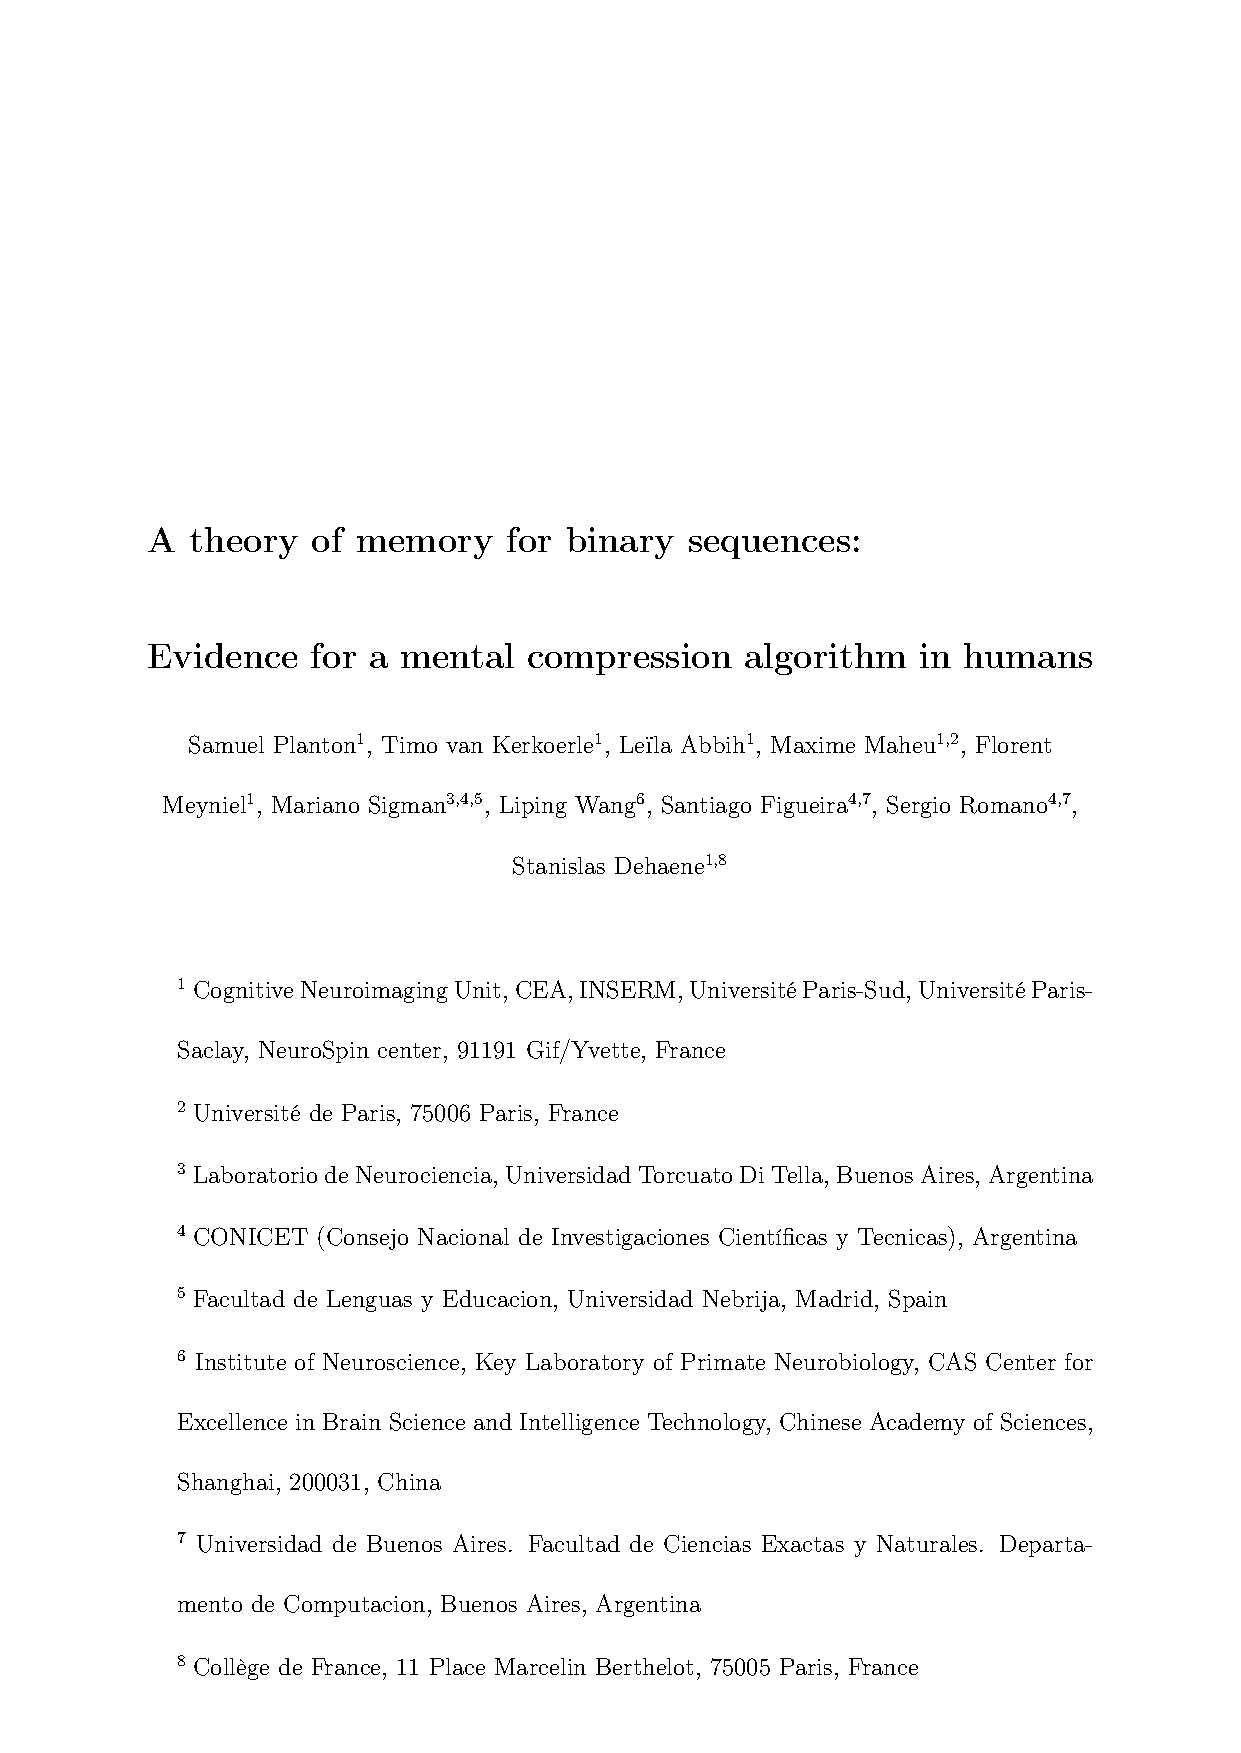
\includepdf[pages=-]{manuscript_pcb.pdf}